\section{Method}
\label{sec:method}

Sparse Readout Prism (SRP) separates two ingredients that are often conflated
in logit-level explanations: the sparse basis learned from the readout rows, and
the scalar score being explained at a particular hidden state. We therefore
first define scalar readout targets, which determine the meaning of support and
opposition, and then introduce the sparse readout factorization used to account
for those targets.

\subsection{Scalar Readout Targets}
\label{sec:problem-setup}

A local score account explains a scalar quantity at a hidden state. Throughout,
``readout'' denotes the final unembedding, or LM head,
\(\WU\in\R^{|\mathcal{V}|\times d}\). For a hidden state \(h\in\R^d\), the row
corresponding to token \(t\) is \(w_t^\top\), so the full logit vector is
\(\WU h\).

We call any linear scalarization of the readout rows a \emph{readout target}.
Formally, let \(\alpha\in\R^{|\mathcal{V}|}\) be a vector of vocabulary-row
coefficients and define
\[
    q_\alpha
    =
    \sum_{t\in\mathcal{V}}\alpha_t w_t,
    \qquad
    s_\alpha(h)
    =
    h^\top q_\alpha .
\]
The standard logit-lens coordinate is recovered as the token-logit special case
\[
    \ell_A(h)=h^\top w_A,
\]
corresponding to \(\alpha_A=1\) and \(\alpha_t=0\) for all \(t\neq A\). SRP can
account for individual token logits directly, but contrastive targets often
reduce sensitivity to shared output-embedding geometry and tokenizer-induced row
structure
\citep{press2017outputembedding,inan2017tying,yang2018softmaxbottleneck,bostrom2020bpe}.

The target choice fixes the question being answered. In a source-verification
example, \(w_{\texttt{verify}}\) asks what raises the \texttt{verify} logit;
\(w_{\texttt{verify}}-\bar{w}_{\mathcal{V}}\) asks what raises it above an
average vocabulary row; \(w_{\texttt{verify}}-w_{\texttt{assume}}\) asks why it
beats a specific alternative; and a local margin compares it with several nearby
competitors. These are distinct readout questions, even though they are all
linear targets.

The remaining targets used in this work are linear contrasts. A pairwise logit
difference,
\[
    m_{A,B}(h)
    =
    h^\top(w_A-w_B),
\]
asks why the readout supports token \(A\) over token \(B\). Because the
coefficients sum to zero, shared offsets cancel and the sign directly encodes
the favored side. For behaviors distributed across multiple tokens, such as
answering, acting, or abstaining, we use group contrasts. For any nonempty token
set \(\mathcal{A}\subseteq\mathcal{V}\), define
\[
    \bar{w}_{\mathcal{A}}
    =
    \frac{1}{|\mathcal{A}|}
    \sum_{a\in\mathcal{A}} w_a .
\]
The group contrast is then
\[
    q_{\mathcal{A},\mathcal{B}}
    =
    \bar{w}_{\mathcal{A}}-\bar{w}_{\mathcal{B}} .
\]
This preserves linearity while reducing dependence on any single tokenizer row.
The vocabulary-mean row
\[
    \bar{w}_{\mathcal{V}}
    =
    \frac{1}{|\mathcal{V}|}
    \sum_{t\in\mathcal{V}} w_t
\]
gives a reference contrast. We also use local margins against nearby
competitors,
\[
    w_u-\sum_{r\in\mathcal{R}}\pi_r w_r,
\]
where \(\mathcal{R}\) is a fixed competitor set and \(\pi\) is a fixed weight
vector over that set. The main target families are therefore token logits,
reference contrasts, pairwise logit differences, group contrasts, and
top-competitor margins.

The scalar \(s_\alpha(h)\) is the unit of a local account. Fixing this target
before applying SRP keeps token preferences, reference contrasts, and decision
margins distinct.

\subsection{Sparse Readout Prism}
\label{sec:method-srp}

Sparse Readout Prism provides a sparse coordinate system for the final readout.
Rather than explaining logits directly in the vocabulary basis, SRP first
factorizes the unembedding rows into sparse token-specific coefficients and
shared decoder directions in hidden-state space. This factorization supports
three linked uses: full LM-head replacement for fidelity tests,
target-independent profiles \(D_{\mathrm{feat}}h\) describing which readout
features are present in a hidden state, and, once a scalar target is fixed,
local signed decompositions of the target score into feature contributions and
residual error.

\begin{figure}[t]
    \centering
    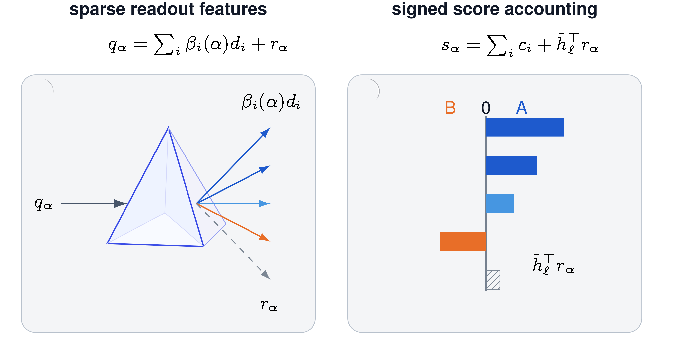
\includegraphics[width=\columnwidth]{figures/schematic_tikz/readout_query_one_column.pdf}
    \vspace{-0.8\baselineskip}
    \caption{\textbf{Local score account schematic.}
    A centered or contrast readout target is decomposed into SAE features learned
    from unembedding rows. For \(w_A-w_B\), \(A\) and \(B\) are the competing
    token or token-set sides: positive bars support \(A\) over \(B\), negative
    bars support \(B\) over \(A\). At hidden state \(h\), each signed term is a
    target coefficient times \(h\)'s projection onto the corresponding readout
    feature; hatching marks reconstruction error. Raw token-logit targets also
    include a shared offset.}
    \label{fig:readout-query-schematic}
\end{figure}

\subsubsection{Raw-Coordinate Readout Factorization}

For each token row \(t\), the readout SAE approximates the corresponding
unembedding vector as
\[
    \widehat{w}_t
    =
    \mu+\sum_{i=1}^{D}z_{t,i}d_i,
    \qquad
    r_t
    =
    w_t-\widehat{w}_t,
\]
where \(\mu\) is a shared offset, \(d_i\in\R^d\) is a decoder direction,
\(z_{t,i}\) is the sparse coefficient of token row \(t\), and \(r_t\) is the
row-reconstruction residual. All score decompositions below are performed after
mapping the fitted representation back to the model's original readout
coordinates. Thus the exact accounting identity used throughout is
\[
    w_t
    =
    \mu+\sum_{i=1}^{D}z_{t,i}d_i+r_t .
\]
Stacking the fitted rows \(\widehat{w}_t^\top\) yields the reconstructed readout
\(\widehat{\WU}\). The only approximation term in later logit or contrast
decompositions is therefore the explicitly reported reconstruction residual.
Appendix~\ref{app:score-accounting} gives the centering and row-normalization
details.

\subsubsection{Learning the Readout Factorization}

We fit TopK readout SAEs \citep{makhzani2013ksparse,gao2024scaling} over
centered, and optionally row-normalized, unembedding rows. Let
\[
    x_t
    =
    \frac{w_t-\mu}{a_t},
\]
where \(a_t=1\) when row normalization is not used. An encoder produces a
\(D\)-dimensional pre-code, retains the \(k\) largest entries, and decodes the
result using directions \(\widetilde d_i\):
\[
    \widetilde z_t
    =
    \operatorname{TopK}_k(f_\theta(x_t)),
    \qquad
    \widehat{x}_t
    =
    \sum_{i=1}^{D}\widetilde z_{t,i}\widetilde d_i .
\]
The training objective is row-wise reconstruction:
\[
    \min_{\theta,\{\widetilde d_i\}}
    \frac{1}{|\mathcal{V}|}
    \sum_{t\in\mathcal{V}}
    \left\|x_t-\widehat{x}_t\right\|_2^2 .
\]
After fitting, we convert the learned quantities back to raw readout space:
\[
    z_{t,i}=a_t\widetilde z_{t,i},
    \qquad
    d_i=\widetilde d_i,
    \qquad
    r_t=a_t(x_t-\widehat{x}_t).
\]
Consequently, all subsequent equations decompose the model's original logits or
contrasts using the raw-coordinate identity above, without adding a separate
dense correction term. The width \(D\) and native sparsity \(k\) are selected by
held-out reconstruction quality and readout-replacement fidelity.
Appendices~\ref{app:readout-factorizer-sweeps}--%
\ref{app:readout-factorizer-diagnostics-reproducibility} provide the selection
overview, recipe sweeps, transfer rows, diagnostics, and reproducibility details.

\subsubsection{Full Readout Replacement and Target-Independent Profiles}

The same factorization applies to the full readout map. Let
\(Z\in\R^{|\mathcal{V}|\times D}\) collect the sparse row codes, and let
\(D_{\mathrm{feat}}\in\R^{D\times d}\) have rows \(d_i^\top\). The reconstructed
LM head and its induced logits are
\[
    \begin{aligned}
    \widehat{\WU}
    &=
    \mathbf{1}\mu^\top
    +
    ZD_{\mathrm{feat}},
    \\
    \widehat{\ell}(h)
    &=
    \widehat{\WU}h
    \\
    &=
    \mathbf{1}(\mu^\top h)
    +
    Z(D_{\mathrm{feat}}h).
    \end{aligned}
\]
Full readout replacement evaluates the global faithfulness of the learned
factorization by measuring how well \(\widehat{\WU}\) preserves LM-head
behavior.

The vector \(D_{\mathrm{feat}}h\) is the target-independent \emph{profile} of
hidden state \(h\). It describes which readout features are present in the
hidden state before any token, contrast, or group comparison is selected. These
profile entries become support or opposition only after multiplication by a row
code or target coefficient. All quantitative reconstructions use the full
feature sum, while visualizations may truncate small bars for readability.

\subsubsection{Local Score Decomposition}

A local account is defined with respect to a particular hidden state \(h\) and a
particular scalar readout target \(q_\alpha\). Substituting the raw-coordinate
SRP identity into \(s_\alpha(h)=h^\top q_\alpha\) gives
\[
\begin{aligned}
    s_\alpha(h)
    &= h^\top q_\alpha \\
    &=
    \left(\sum_{t\in\mathcal{V}}\alpha_t\right)h^\top\mu \\
    &\quad+
    \sum_{i=1}^{D}
    \left(\sum_{t\in\mathcal{V}}\alpha_t z_{t,i}\right)h^\top d_i \\
    &\quad+
    h^\top\sum_{t\in\mathcal{V}}\alpha_t r_t .
\end{aligned}
\]
For feature \(i\), define its target coefficient and SRP contribution as
\[
    \beta_i(\alpha)
    =
    \sum_{t\in\mathcal{V}}\alpha_t z_{t,i},
    \qquad
    c_i(h,\alpha)
    =
    \beta_i(\alpha)\,h^\top d_i .
\]
This product form is the central separation in SRP:
\(\beta_i(\alpha)\) is a readout-side factor determined only by the chosen
target and the learned LM-head factorization, while \(h^\top d_i\) is a
context-side factor determined only by the current hidden state. A feature
matters locally when both factors are large. Positive contributions raise the
chosen scalar score, whereas negative contributions lower it. The projection
\(h^\top d_i\) alone belongs to the target-independent profile
(Appendix~\ref{app:global-readout-feature-activations}); target coefficients
turn profile activations into token- or contrast-specific evidence.

Let
\[
    s_\mu
    =
    \left(\sum_{t\in\mathcal{V}}\alpha_t\right)h^\top\mu,
    \qquad
    s_{\mathrm{feat}}
    =
    \sum_i c_i(h,\alpha),
    \qquad
    s_{\mathrm{recon}}
    =
    s_\mu+s_{\mathrm{feat}} .
\]
The local reconstruction error is
\[
    \epsilon
    =
    s_{\mathrm{exact}}-s_{\mathrm{recon}}
    =
    h^\top\sum_{t\in\mathcal{V}}\alpha_t r_t .
\]
Thus the feature bars are faithful to the chosen scalar score when
\(|\epsilon|\) is small, and the residual explicitly marks any unexplained
component. Figures report the original target score, feature sum, offset when
present, and reconstruction error alongside signed contribution bars. For
signed contrasts, sign-preserved reconstructions give directly readable support
and opposition. Appendix~\ref{app:score-accounting} states the full identities.

\subsubsection{Common Target Coefficients}

The same identity covers the target families from \Cref{sec:problem-setup}.
\Cref{tab:method-special-cases} instantiates the general target \(q_\alpha\) and
the corresponding feature coefficient \(\beta_i(\alpha)\). For compactness,
write
\[
    \bar{z}_{\mathcal{A},i}
    =
    \frac{1}{|\mathcal{A}|}
    \sum_{a\in\mathcal{A}}z_{a,i}
\]
for the uniform average of feature \(i\)'s sparse coefficient over token group
\(\mathcal{A}\). For top-competitor margins, write
\[
    \bar{w}_{\pi,\mathcal{R}}
    =
    \sum_{r\in\mathcal{R}}\pi_r w_r,
    \qquad
    \bar{z}_{\pi,\mathcal{R},i}
    =
    \sum_{r\in\mathcal{R}}\pi_r z_{r,i}.
\]

\begin{table}[tbp]
\caption{\textbf{Scalar readout target coefficients.}
Rows instantiate the general target \(q_\alpha\) and the corresponding SAE
feature coefficient \(\beta_i(\alpha)\). Barred quantities denote uniform
token-set averages or competitor-weighted averages.}
\label{tab:method-special-cases}
\centering
\footnotesize
\setlength{\tabcolsep}{3pt}
\renewcommand{\arraystretch}{1.14}
\begin{tabularx}{\linewidth}{@{}>{\RaggedRight\arraybackslash}p{0.34\linewidth}Z Z@{}}
\toprule
Target & \(q_\alpha\) & \(\beta_i(\alpha)\) \\
\midrule
\textbf{Token score} & \(w_A\) & \(z_{A,i}\) \\
\addlinespace[1pt]
\textbf{Reference contrast} & \(w_A-\bar{w}_{\mathcal{V}}\) &
\(z_{A,i}-\bar{z}_{\mathcal{V},i}\) \\
\addlinespace[1pt]
\textbf{Logit difference} & \(w_A-w_B\) & \(z_{A,i}-z_{B,i}\) \\
\addlinespace[1pt]
\textbf{Group contrast} &
\(\bar{w}_{\mathcal{A}}-\bar{w}_{\mathcal{B}}\) &
\(\bar{z}_{\mathcal{A},i}-\bar{z}_{\mathcal{B},i}\) \\
\addlinespace[1pt]
\textbf{Local competitor} &
\(w_u-\bar{w}_{\pi,\mathcal{R}}\) &
\(z_{u,i}-\bar{z}_{\pi,\mathcal{R},i}\) \\
\bottomrule
\end{tabularx}
\end{table}

For reference contrasts, pairwise logit differences, group contrasts, and
competitor margins, the target coefficients sum to zero and the shared offset
cancels. Positive values support the first side of the comparison, while
negative values support the reference or competitor side. Other reference
targets use the same formula with their corresponding reference coefficients.

Contribution-plot labels summarize the vocabulary rows most associated with a
feature; the measured quantities are the feature id and signed contribution.
Because unembedding rows reflect both semantic and tokenizer-induced structure,
we treat feature labels as descriptive summaries rather than ground-truth
semantics. Following sparse-feature evaluation practice
\citep{karvonen2025saebench,makelov2024principled}, appendix controls report
tokenization, row-norm, frequency, special-token, and feature-labeling metadata.